\Large\textbf{Capitolo 2: \\ Funzioni e struttura delle proteine}

\section{Struttura gerarchica}
    \small
    L'intero insieme di proteine che può essere espresso dall'organismo prende il nome di \textbf{proteoma}. Il genoma consente di identificare molte più proteine rispetto a quelle effettivamente espresse.
    Le proteine si classificano in 
    \begin{itemize}
        \item dipeptidi: composti da due amminoacidi (AA)
        \item oligopeptidi: composti da meno di 20/30 AA
        \item polipeptidi: composti da 200/500 AA 
    \end{itemize}
    Gli AA di cui si compongono le proteine si dividono nelle seguenti categorie 
    \begin{itemize}
        \item non polari
        \item polari, che a loro volta si dividono in: 
        \begin{itemize}
            \item carichi positivamente
            \item carichi negativamente
            \item neutri
        \end{itemize}
    \end{itemize}
    Gli AA sono legati l'un l'altro tramite legami peptidici, la reazione che porta al legame è una reazione di consensazione (CREDO). La catena amminoacidica si legge a partire dall'AA che espone l'N-terminale fino all'AA che espone il C-terminale (perchè corrisponde all'ordine di sintesi del peptide).\\
    Ogni proteina sintetizzata assume una conformazione tridimensionale dovuti alle interazioni elettrostatiche tra gli AA. L'urea è una molecola che destabilizza la formazione di questi legami. Ci sono enzimi (chaperon) che concorrono alla formazione della conformazione tridimensionale corretta.
    
          \begin{figure}[h]
            \centering
            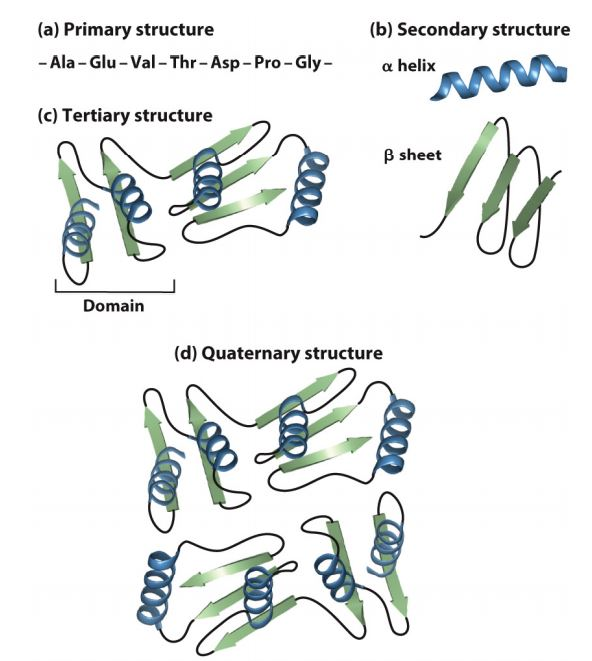
\includegraphics[width=0.5\textwidth]{images/proteinegerarchia.JPG}
            \caption{\small schema generale delle strutture proteiche}
            \label{fig:mesh1}
        \end{figure}
    
    \subsection{Folding}
        \small
        Per \textbf{Folding} si intende il processo di ripiegamento della catena amminoacidica. Questo evento consiste nella formazione di legami (solitamente legami a idrogeno) tra le catene laterali degli AA o il backbone della catena amminoacidica stessa (tutte le combinazioni sono possibili).
        Le ripiegature scorrette possono essere la causa di patologie (per esempio il morbo della mucca pazza).
    
        \subsubsection{Eccezioni}
            In alcuni casi il folding può avvenire tramite interazioni non-covalenti, nonostante ciò si instaurano legami covalenti tra catene polipeptidiche diverse (anche tra le catene laterali dello stesso polipeptide) (?)\\
            
            \textbf{Ponte di-solfuro}  \\
            Il ponte di solfuro si forma su due cisteine, che consolidano interazioni non-covalenti all'interno della cellula cosicché possa mantenere la stessa stabilità all'esterno.
            Esempio: in un anticorpo, le catene pesanti e leggere presentano ponti di-solfuro tra per stabilizzare la molecola.
    
    
    \subsection{Struttura primaria}
        La struttura primaria della proteina consiste nella sequenza amminoacidica di cui è composta, è polarizzata (?) e si considera il primo AA quello che espone l'N-terminale.
    
    
    \subsection{Struttura secondaria}
        La struttura secondaria consiste in ripiegamenti locali della sequenza di AA. Le due strutture secondarie che si riscontrano sono $\alpha -Elica$ ($\alpha E$) e $\beta -Foglietto$ ($\beta F$). 
        
        \subsubsection{$\alpha -Elica$}
            L'$\alpha E$ è un organizzazione 3D che consiste nella disposizione dei residui AA verso l'esterno, è resa stabile per i legami H tra gli atomi del backbone. 
            La sia struttura risulta sempre uguale a se stessa indipendentemente dai residui AA (un ossigeno si lega sempre ad un idrogeno dell'AA quattro posizioni più avanti). Il passo dell'elica corrisponde a 0.54 nm. Per compiere un giro sono necessari 3.6 AA.\\
            Alcuni AA interferiscono con la formazione della struttura, in particolare glicina e prolina.\\
            L'$\alpha E$ può assumere proprietà chimiche differenti a seconda della sequenza AA che la compone. Per esempio può contenere code idrofobiche nel caso l'$\alpha E$ sia destinata a fare parte di un complesso proteico trans-membrana.
            Può essere destrorsa o sinistrorsa.
        
        \subsubsection{$\beta -Foglietto$}
            Il $\beta F$ è basato sulle interazioni H tra gli atomi del backbone. Le catene laterali degli AA sono disposte alternativamente sopra e sotto il piano del foglietto. Anche in questo caso, la sua struttura è indipendente dalla catena AA ed è sempre uguale a se stessa. \\
            Gli \textit{strand} del foglio possono essere orientati in maniera:
            \begin{itemize}
                \item parallela (da un lato del foglietto si trovano tutti gli N-terminali)
                \item antiparallela (l'N-terminale si alterna tra i lati del foglio). 
                Viene chiamato $\beta -turn$ il ripiegamento che connette due filamenti antiparalleli, ha una composizione sistematica di 4 AA.
            \end{itemize}
            Esistono strutture ibride (porzioni parallele e antiparallele).
        
    
    \subsection{Struttura terziaria}
        Per struttura terziaria si intendono ripiegamenti di porzioni più ampie della sequenza AA. 
        
        \subsubsection{Coled-coil motiv}
            La struttura del Coiled-coil si può formare in presenza di due $\alpha E$ che si "arrotolano" su loro stesse. Le eliche che tendono a formare questa struttura comprendono delle sequenze AA specifiche chiamate \textit{heptad repeat} lunghe sette AA. 
            Le posizioni interne a questa sequenza sono spesso indicate con \textit{abcdefg} dove \textit{a} e \textit{d} sono AA idrofobici (1 e 4).
            Le due eliche, avendo caratteristiche simili, tendono ad associarsi per stabilizzarsi. Non si ripiegano necessariamente l'una sull'altra autonomamente.
        
        \subsubsection{Domini}
            Un dominio è una porzione della proteina che comprende più strutture secondarie e assumono una conformazione autonomamente.
        
        \subsubsection{Domini non strutturati}
            Un dominio non strutturato non assume conformazione propria, ma possono interagire con altre molecole per assumere una conformazione specifica. Possono svolgere una funzione di signaling o regolatoria.\\
            
            \textbf{Chaperon}\\
            Il folding di una proteina avviene infatti contemporaneamente alla sintesi, qualora la conformazione 3D attesa debba passare attraverso uno stato energicamente sfavorito, può intervenire uno \textit{Chaperon}, che collabora alla formazione della proteina matura.
        
    
    \subsection{Struttura quaternaria}
        Per struttura quaternaria si intende l'associazione di più polipeptidi per la formazione di un complesso funzionale. 
        Le proteine formate tendono ad assumere conformazioni standard (le conformazioni che effettivamente si riscontrano sono una piccola percentuale rispetto al totale delle combinazioni per un determinato numero di AA).\\
        Le associazioni tra polipeptidi differenti avvengono attraverso legami non-covalenti per la formazione di polimeri. Esistono degli agenti che permettono l'aggregazione di una molecola funzionante (?).
        
     
    
\section{Funzioni}
    Le funzioni delle proteine possono essere talvolta già associate ad una struttura terziaria. In alcuni casi il ruolo di un polipeptide è funzionale ad un complesso strutturalmente più complesso (ad esempio il ribosoma). \\
    Le funzioni principali delle proteine sono:
    \begin{enumerate}
        \item regolatoria
        \item strutturale
        \item movimento della cellula
        \item enzimatica
        \item trasporto
        \item signaling
    \end{enumerate}
    
    
    \pagebreak